%Chapter 3
\chapter{3}{Ekvationer och olikheter}
\subsection*{Ekvationer}

\begin{task}{3.1 a)}
	Utnyttja faktorsatsen (varje faktor är ett nollställe).
	
	\ans $x_1=1$, $x_2=2$, $x_3=3$
\end{task}

\begin{task}{b)}
	$x(x^2-4)=0$. Faktorisera först $x^2-4$ med konjugatregeln.
	\[x(x+2)(x-2)=0\]
	Utnyttja sedan faktorsatsen (varje faktor är ett nollställe).
	
	\ans $x_1=0$, $x_2=-2$, $x_3=2$
\end{task}

\begin{task}{c)}
	\[x^2+10x+24=0\]
	\emph{Alternativ 1:}
	
	Faktorisera genom att gissa $a$ och $b$ så $(x+a)(x+b)=x^2+10x+24=0$. $a = 4$ och $b = 6$.
	\[(x+4)(x+6)=0\]
	Utnyttja sedan faktorsatsen (varje faktor är ett nollställe).
	
	\emph{Alternativ 2:}
	
	Använd pq-formeln:
	
	\[x=-5\pm\sqrt{5^2-24}=-5\pm 1\]
	\emph{Alternativ 3:}
	
	Använd kvadratkomplettering:
	\[(x+5)^2-25+24=0 \lra (x+5)^2=1 \lra x+5=\pm \sqrt{1} \lra x=-5\pm 1\]
	\ans $x_1=-4$ och $x_2=-6$
\end{task}

\begin{task}{d)}
	\[x^2+10x+25=0\]
	\emph{Alternativ 1:}
	
	Faktorisera genom att gissa $a$ och $b$ så $(x+a)(x+b)=x^2+10x+25=0$. $a = 5$ och $b = 5$.
	\[(x+5)^2=0\]
	Utnyttja sedan faktorsatsen (varje faktor är ett nollställe).
	
	\emph{Alternativ 2:}
	
	Använd pq-formeln:
	
	\[x=-5\pm\sqrt{5^2-25}=-5\pm \sqrt{0}=-5\]
	\emph{Alternativ 3:}
	
	Använd kvadratkomplettering:
	\[(x+5)^2-25+25=0 \lra (x+5)^2=0 \lra x+5=0 \lra x=-5\]
	\ans $x_{1,2}=-5$
\end{task}

\begin{task}{e)}
	\[x^3+10x^2+24x=0\]
	
	Faktorisera ut $x$ ur vänsterledet.
	\[x(x^2+10x+24)=0\]
	Hitta nollställena till $x^2+10x+24$ (se \taskref{c)}). Nollproduktionsmetoden ger också lösningen $x=0$.
	
	\ans $x_1=-4$, $x_2=-6$ och $x_3=0$
\end{task}

\begin{task}{f)}
	\[x^4+10x^3+25x^2=0\]
	
	Faktorisera ut $x^2$ ur vänsterledet.
	\[x^2(x^2+10x+25)=0\]
	Hitta nollställena till $x^2+10x+25$ (se \taskref{d)}). Nollproduktionsmetoden ger också dubbelroten $x=0$.
	
	\ans $x_{1,2}=-5$ och $x_{3,4}=0$
\end{task}

\begin{task}{3.2 a)}
	\[x^2+4x+a=0,~~x=2\]
	Sätt in värdet för $x$ i ekvationen och lös ut $a$.
	\[2^2+4\*2+a=0\lra 4+8+a=0\lra a=-12\]
	\ans $a=-12$
\end{task}

\begin{task}{b)}
	\[x^2+bx+12=0,~~x=3\]
	Sätt in värdet för $x$ i ekvationen och lös ut $b$.
	\[3^2+3b+12=0\lra 9+3b+12=0\lra 3b=-21 \lra b=-7\]
	\ans $b=-7$
\end{task}

\begin{task}{3.3 a)}
	\[p(x)=x^2-x-\frac{3}{4}\]
	\[x^2-x-\frac{3}{4}=0\]
	Använd pq-formeln (eller kvadratkomplettering).
	\[x=\frac{1}{2}\pm\sqrt{\frac{1}{4}+\frac{3}{4}}=\frac{1}{2}\pm 1 \ra x_1=\frac{3}{2},~~x_2=-\frac{1}{2}\]
	Faktorsatsen ger: $p(x)=(x-\frac{3}{2})(x+\frac{1}{2})$
	
	\ans $p(x)=\left(x-\dfrac{3}{2}\right)\left(x+\dfrac{1}{2}\right)$
\end{task}

\begin{task}{b)}
	\[p(x)=2x^2-3x-2\]
	\[2x^2-3x-2=0 \lra x^2-\frac{3}{2}x-1=0\]
	Använd pq-formeln (eller kvadratkomplettering).
	\[x=\frac{3}{4}\pm\sqrt{\left(\frac{3}{4}\right)^2+1}=
	\frac{3}{4}\pm\sqrt{\frac{9}{16}+\frac{16}{16}}=
	\frac{3}{4}\pm \frac{5}{4}
	\ra x_1=2,~~x_2=-\frac{1}{2}\]
	Faktorsatsen ger: $p(x)=(x-2)(x+\frac{1}{2})$
	
	\ans $p(x)=\left(x-2\right)\left(x+\dfrac{1}{2}\right)$
\end{task}

\begin{task}{c)}
	\[p(x)=-x^2+x+12\]
	\[-x^2+x+12=0 \lra x^2-x-12=0\]
	Använd pq-formeln (eller kvadratkomplettering).
	\[x=\frac{1}{2}\pm\sqrt{\frac{1}{4}+12}=
	\frac{1}{2}\pm\sqrt{\frac{1}{4}+\frac{48}{4}}=
	\frac{1}{2}\pm \frac{7}{2}
	\ra x_1=4,~~x_2=-3\]
	Faktorsatsen ger: $p(x)=(x-4)(x+3)$
	
	\ans $p(x)=(x-4)(x+3)$
\end{task}

\begin{task}{d)}
	\[p(x)=x^3-x^2+\frac{1}{4}x=x\left(x^2-x+\frac{1}{4}\right)\]
	\[g(x)=x^2-x+\frac{1}{4}\]
	\[x(x^2-x+\frac{1}{4})=0 \lra x\*g(x)=0\]
	Använd pq-formeln (eller kvadratkomplettering) på $g(x)=0$.
	\[x=\frac{1}{2}\pm\sqrt{\frac{1}{4}-\frac{1}{4}}=
	\frac{1}{2}\pm 0=
	\frac{1}{2}
	\ra x_{1,2}=\frac{1}{2}\]
	Faktorsatsen ger: $g(x)=(x-\frac{1}{2})^2$
	\[p(x)=x\*g(x)=x(x-\tfrac{1}{2})^2\]
	\ans $p(x)=x\left(x-\dfrac{1}{2}\right)^2$
\end{task}

\begin{task}{e)}
	\[p(x)=3x^3-6x^2+15x=3x(x^2-2x+5)\]
	\[g(x)=x^2-2x+5\]
	\[x(x^2-2x+5)=0 \lra x\*g(x)=0\]
	Använd pq-formeln (eller kvadratkomplettering) på $g(x)=0$.
	\[x=1\pm\sqrt{1-5} \ra \text{Saknar reell lösning}\]
	Faktorsatsen ger då att $g(x)$ inte kan faktoriseras.
	
	\ans $p(x)=3x(x^2-2x+5)$
\end{task}

\begin{task}{f)}
	\[p(x)=x^4-6x^2+8\]
	Använd variabelsubstitution så pq-formeln kan användas.
	\[x^4-6x^2+8=0,~~t=x^2 \ra t^2-6t+8=0\]
	Använd pq-formeln (eller kvadratkomplettering).
	\[t=3\pm\sqrt{9-8} \lra t=3\pm 1 \ra t_1=4,~~t_2=2\]
	\[x^2=4 \lra x_{1,2}=\pm 2\]
	\[x^2=2 \lra x_{3,4}=\pm \sqrt{2}\]
	Faktorsatsen ger då $p(x)=(x-2)(x+2)(x-\sqrt{2})(x+\sqrt{2})$
	
	\ans $p(x)=(x-2)(x+2)(x-\sqrt{2})(x+\sqrt{2})$
\end{task}

\begin{task}{3.4}
	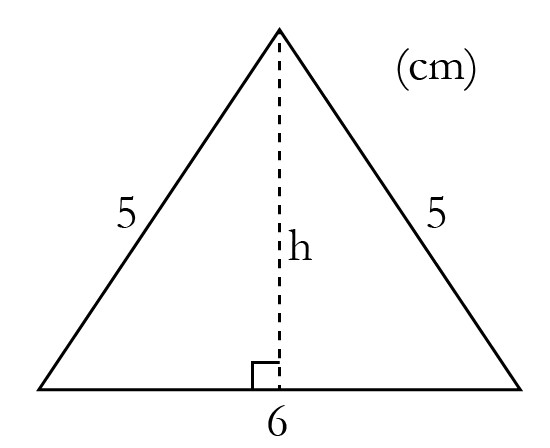
\includegraphics[scale=0.3]{images/34.PNG}
	
	Satsen om likbent triangel ger att båda rätvinkliga trianglarna är kongruenta vilket medför att basen för båda är $3\text{cm}$.
	Pyth. sats ger att $h=\sqrt{5^2-3^2}=4 \ra$ arean: $6\*4/2=12\text{cm}^2$ och omkretsen är $16\text{cm}$.
	
	Låt benen vara $y$ och basen $h=\sqrt{y^2-(x/2)^2}$ 
	
	area: $\dfrac{x\*h}{2}=\dfrac{x\sqrt{y^2-(x/2)^2}}{2}=12cm \lra x\sqrt{y^2-(x/2)^2}=24\text{cm}$ 
	
	omkrets: $2y+x=16\text{cm} \lra x=16-2y$
	\begin{align*}
	&(16-2y)\sqrt{y^2-(8-y)^2}=24 \lra
	2(8-y)4\sqrt{y-4}=24 \lra \\ \lra
	&(8-y)\sqrt{y-4}=3 \ra
	(y^2-16y+64)(y-4)=9 \lra \\ \lra
	&y^3-4y^2-16y^2+64y+64y-256=9 \lra
	y^3-20y^2+128y-265=0
	\end{align*}
	Ansätter lösning med $x-5$ som faktor från ursprungsfiguren (kan lösas med polynomdivision också):
	\[y^3-20y^2+128y-265=(y-5)(y^2+Ay+B)=y^3+(A-5)y^2+(B-5A)y-5B\]
	Identifierar variablerna:
	\[\begin{cases}
	A-5=-20 \\
	B-5A=128
	\end{cases}
	\lra
	\begin{cases}
	A=-15 \\
	B=53
	\end{cases}\]
	\[y^3-20y^2+128y-265=(y-5)(y^2-15y+53)\]
	\[y^2-15y+53=0\]
	pq-formeln:
	\[y=\dfrac{15}{2}\pm\sqrt{\dfrac{15^2-212}{4}}=\dfrac{15\pm\sqrt{13}}{2}\]
	\[y_1=\dfrac{15+\sqrt{13}}{2} \ra
	x=16-15-\sqrt{13} \ra
	x < 0 \ra\text{ falsk rot}\]
	\[y_2=\dfrac{15-\sqrt{13}}{2} \ra x=16-15+\sqrt{13}=1+\sqrt{13}\]
	\ans $x=1+\sqrt{13}$ och $y=\dfrac{15-\sqrt{13}}{2}$
\end{task}

\begin{task}{3.5 a)}
	\begin{align*}
	&\dfrac{1}{x-1}+\dfrac{1}{x}+\dfrac{1}{x+1}=0\lra
	\dfrac{x(x+1)+x^2-1+x(x-1)}{x(x^2-1)}=0 \lra \\ \lra
	&\dfrac{3x^2-1}{x(x^2-1)}=0\ra
	3x^2-1=0 \lra
	(\sqrt{3}x+1)(\sqrt{3}x-1)=0 \lra \\ \lra
	&\left(x+\frac{1}{\sqrt{3}}\right)\left(x-\frac{1}{\sqrt{3}}\right)=0
	\end{align*}
	Faktorsatsen ger då: $x_1=-\frac{1}{\sqrt{3}}$ och $x_2=\frac{1}{\sqrt{3}}$
	
	\ans $x_{1,2}=\pm\frac{1}{\sqrt{3}}$
\end{task}

\begin{task}{b)}
	\begin{align*}
	&\dfrac{1}{x-1}-\dfrac{1}{x-2}=\dfrac{1}{x-3}-\dfrac{1}{x-4}\lra
	\dfrac{\cancel{x}-2-\cancel{x}+1}{(x-1)(x-2)}=\dfrac{\cancel{x}-4-\cancel{x}+3}{(x-3)(x-4)} \lra \\ \lra
	&\dfrac{1}{x^2-3x+2}=\dfrac{1}{x^2-7x+12} \ra
	\cancel{x^2}-3x+2=\cancel{x^2}-7x+12 \lra \\ \lra
	&x=\frac{10}{4}=\frac{5}{2}
	\end{align*}
	\ans $x=\frac{5}{2}$
\end{task}

\begin{task}{c)}
	\begin{align*}
	&\dfrac{1}{x^2-2x}+\dfrac{1}{x^2+3x}=0 \lra
	\dfrac{\cancel{x}(x+3)+\cancel{x}(x-2)}{x^{\cancel{2}}(x-2)(x+3)}=0 \ra \\ \ra
	&x+3+x-2=0 \lra
	2x+1=0 \lra
	x=-\frac{1}{2}
	\end{align*}
	\ans $x=-\frac{1}{2}$
\end{task}

\begin{task}{d)}
	\begin{align*}
	&\dfrac{1}{x+2}-\dfrac{x+2}{x-2}=\dfrac{x^2}{4-x^2}\lra
	\dfrac{x-2-(x+2)^2}{x^2-4}=\dfrac{x^2}{4-x^2} \ra \\ \ra
	&(4-x^2)(-x^2-3x-6)=x^2(x^2-4) \lra \\ \lra
	&-\cancel{4x^2}-12x-24+\cancel{x^4}+3x^3+6x^2=\cancel{x^4}-\cancel{4x^2} \lra \\ \lra
	&x^3+2x^2-4x-8=0
	\end{align*}
	Gissar en lösning till ekvationen och hittar $x=2$. Ansätter lösning med $x-2$ som faktor (kan lösas med polynomdivision också):
	\[x^3+2x^2-4x-8=(x-2)(x^2+Ax+B)=x^3+(A-2)x^2+(B-2A)x-2B\]
	Identifierar variabler:
	\[\begin{cases}
	A-2=2 \\
	B-2A=-4
	\end{cases}
	\lra
	\begin{cases}
	A=4 \\
	B=4
	\end{cases}\]
	\[(x-2)(x^2+4x+4)=0\]
	Kvadreringsregeln:
	\[(x-2)(x^2+4x+4)=0\lra
	(x-2)(x+2)^2=0\]
	Faktorsatsen: $x_1=2$ och $x_{2,3}=-2$.
	Både $2$ och $-2$ är dock falska rötter då de resulterar i nolldivision i ursprungsekvationen.
	
	\ans Ekvationen saknar lösning
\end{task}

\begin{task}{3.6}
	Formeln för hastighet, sträcka och tid är $s=v\*t \lra t=\frac{s}{v}$. Låt $x$ vara båtens hastighet i stillastående vatten. Den totala tiden för resan är tiden dit ($t_1$) plus tiden tillbaka ($t_1$) ($t_1+t_2=t$).
	Hastigheten båten har dit ($v_1$) kan beskrivas som $x-2.4$ och hastigheten hem ($v_2$) som $x+2.4$. $t=2$ och $s=6.4$.
	\[t_1+t_2=t\lra
	\frac{s}{v_1}+\frac{s}{v_2}=t\]
	\begin{align*}
	&\frac{6.4}{x-2.4}+\frac{6.4}{x+2.4} = 2 \lra
	\frac{6.4(x+2.4)+6.4(x-2.4)}{(x-2.4)(x+2.4)} = 2 \lra \\ \lra
	&6.4(2x+\cancel{2.4-2.4})=2(x^2-2.4^2) \lra
	\cancel{2}\*6.4x=\cancel{2}(x^2-2.4^2) \lra \\ \lra
	&x^2-6.4x-5.76=0
	\end{align*}
	pq-formeln:
	\[x=3.2\pm\sqrt{10.24+5.76} =3.2\pm\sqrt{16}=3.2\pm 4\]
	$x_1=7.2$ och $x_2=-0.8$. Eftersom hastigheten i uppgiften inte kan vara negativ gäller endast $x_1$.
	
	\ans $7.2$ km/h
\end{task}

\begin{task}{3.7 a)}
	\[\sqrt{x+2}=x \ra
	x+2=x^2 \lra
	x^2-x-2=0 \]
	pq-formeln:
	\[x=\frac{1}{2}\pm\sqrt{\frac{1}{4}+\frac{8}{4}} \lra
	x=\frac{1}{2}\pm\frac{3}{2}\]
	$x_1=2$
	
	$x_2=-1$ Falsk rot (sätt in i ursprungsekvationen).
	
	\ans $x=2$
\end{task}

\begin{task}{b)}
	\[\sqrt{x+2}=-x \ra
	x+2=x^2 \lra
	x^2-x-2=0\]
	pq-formeln:
	\[x=\frac{1}{2}\pm\sqrt{\frac{1}{4}+\frac{8}{4}} \lra
	x=\frac{1}{2}\pm\frac{3}{2}\]
	$x_1=2$ Falsk rot (sätt in i ursprungsekvationen).
	
	$x_2=-1$
	
	\ans $x=-1$
\end{task}

\begin{task}{c)}
	\begin{align*}
	&x-\sqrt{x-2}=4 \lra
	\sqrt{x-2}=x-4 \ra
	x-2=(x-4)^2 \lra \\ \lra
	&x-2=x^2-8x+16 \lra
	x^2-9x+18=0
	\end{align*}
	pq-formeln: 
	\[x=\frac{9}{2}\pm\sqrt{\frac{81}{4}-\frac{72}{4}} \lra
	x=\frac{9}{2}\pm\frac{3}{2}\]
	$x_1=6$
	
	$x_2=3$ Falsk rot (sätt in i ursprungsekvationen).
	
	\ans $x=6$
\end{task}

\begin{task}{3.8 a)}
	\[\sqrt{x+2}=\sqrt{2x+1} \ra
	x+2=2x+1 \lra
	x=1\]
	\ans $x=1$
\end{task}

\begin{task}{b)}
	\[\sqrt{3x+2}=\sqrt{2x+1} \ra
	3x+2=2x+1 \lra
	x=-1 \text{\quad Falsk rot.}\]
	\ans Ekvationen saknar lösning
\end{task}

\begin{task}{c)}
	\[\sqrt{x+2}=\sqrt{x} \ra
	x+2=x \lra
	2=0 \text{\quad Ej ekvivalent.}\]
	\ans Ekvationen saknar lösning
\end{task}

\begin{task}{d)}
	\[\sqrt{x-2}\sqrt{x+3}=x \ra
	(x-2)(x+3)=x^2 \lra
	\cancel{x^2}+x-6=\cancel{x^2} \lra
	x=6\]
	\ans $x=6$
\end{task}

\begin{task}{e)}
	\begin{align*}
	&(3-\sqrt{x})(3+\sqrt{x})=8\sqrt{x} \lra
	9-x=8\sqrt{x} \ra \\ \ra
	&x^2-18x+81=64x \lra
	x^2-82x+81=0
	\end{align*}
	pq-formeln:
	\[x=41\pm\sqrt{41^2-81}=41\pm40\]
	$x_1=81$ falsk rot.
	
	$x_2=1$
	
	\ans $x=1$
\end{task}

\begin{task}{f)}
	\begin{align*}
	&\sqrt{x}=\dfrac{3}{\sqrt{x}}+\sqrt{3+x} \lra
	x=3+\sqrt{x(3+x)} \lra
	x-3=\sqrt{3x+x^2} \ra \\ \ra
	&\cancel{x^2}-6x+9=3x+\cancel{x^2} \lra
	9x=9 \lra
	x=1 \text{\quad Falsk rot.}
	\end{align*}
	\ans Lösning saknas
\end{task}

\subsection*{Ekvationer}

\begin{task}{3.9}
	$2<3 \Leftarrow$ är ''2 \textbf{mindre} än 3''? Ja
	
	$2 \le 3 \Leftarrow$ är ''2 \textbf{mindre} eller lika med 3''? Ja
	
	$2 \le 2 \Leftarrow$ är ''2 mindre eller \textbf{lika med} 2''? Ja
	
	\ans Alla tre
\end{task}

\begin{task}{3.10}
	Nedan visar jag min tankeprocess för att lösa uppgiften.
	\[\frac{2}{0.02}=
	\frac{2}{2}\*\frac{1}{10^{-2}}=
	1\*10^2=
	100\]
	\[\frac{31}{0.2}=
	\frac{31}{2}\*\frac{1}{10^{-1}}=
	15.5\*10=
	155\]
	\[\frac{0.00009}{0.000006}=
	\frac{9}{6}\*\frac{10^{-5}}{10^{-6}}=
	1.5\*10=
	15\]
	\ans $\dfrac{0.00009}{0.000006}<\dfrac{2}{0.02}<\dfrac{31}{0.2}$
\end{task}

\begin{task}{3.11 a)}
	$3x+1<2 \lra
	3x<1 \lra
	x<\frac{1}{3}$
	
	\ans $x<\frac{1}{3}$
\end{task}

\begin{task}{b)}
	$-3x+2\le1 \lra
	-3x\le-1 \lra
	x\ge\frac{1}{3}$
	
	\ans $x\ge\frac{1}{3}$
\end{task}

\begin{task}{c)}
	$3x+1>4x+5 \lra
	x<-4$
	
	\ans $x<-4$
\end{task}

\begin{task}{d)}
	$(x-3)(x+3)\le x^2 \lra
	\cancel{x^2}-9 \le \cancel{x^2} \lra
	-9 \le 0 \ra x\in\mathbb{R}$
	
	\ans $x\in\mathbb{R}$
\end{task}

\begin{task}{3.12 a)}
	Använd en teckentabell och hitta intervallet/n som ger positiva värden.
	\[\dfrac{x+4}{x-1}>0\]
	\begin{tabular}{c|c|c|c|c|c}
		$x$ & & $-4$ & & $1$ & \\ \hline
		$x+4$              & $-$ & $0$ & $+$ & $+$ & $+$ \\
		$x-1$              & $-$ & $-$ & $-$ & $0$ & $+$ \\ \hline
		$\dfrac{x+4}{x-1}$ & $+$ & $0$ & $-$ &$\wr$& $+$
	\end{tabular}

	\ans $x>1$ eller $x<-4$
\end{task}

\begin{task}{b)}
	Utnyttja teckentabellen i förra uppgiften men ta intervallet som ger negativa värden.
	\[\dfrac{x+4}{x-1}<0\]
	\ans teckentabellen i \taskref{a)} ger: $-4<x<1$
\end{task}

\begin{task}{c)}
	Använd en teckentabell och hitta intervallet/n som ger negativa värden.
	\[\dfrac{x+1}{x(x-1)}<0\]
	\begin{tabular}{c|c|c|c|c|c|c|c}
		$x$ & & $-1$ & & $0$ & & $1$ & \\ \hline
		$x+1$                  & $-$ & $0$ & $+$ & $+$ & $+$ & $+$ & $+$ \\
		$x$                    & $-$ & $-$ & $-$ & $0$ & $+$ & $+$ & $+$ \\
		$x-1$                  & $-$ & $-$ & $-$ & $-$ & $-$ & $0$ & $+$ \\ \hline
		$\dfrac{x+1}{x(x-1)}$  & $-$ & $0$ & $+$ &$\wr$& $-$ &$\wr$& $+$ \\
	\end{tabular}
	
	\ans $x<-1$ eller $0<x<1$
\end{task}

\begin{task}{d)}
	Använd en teckentabell och hitta intervallet/n som ger positiva värden.
	\[(x+2)(2x-1) > 0\]
	\begin{tabular}{c|c|c|c|c|c}
		$x$ & & $-2$ & & $1/2$ & \\ \hline
		$x+2$         & $-$ & $0$ & $+$ & $+$ & $+$ \\
		$2x-1$        & $-$ & $-$ & $-$ & $0$ & $+$ \\ \hline
		$(x+2)(2x-1)$ & $+$ & $0$ & $-$ &$\wr$& $+$
	\end{tabular}
	
	\ans $x<-2$ eller $x>1/2$
\end{task}

\begin{task}{3.13}
	Skriv om olikheten så att högerledet blir noll och allt i vänsterledet hamnar på samma bråkstreck. Använd sedan en teckentabell och hitta intervallet/n som ger negativa värden.
	\[\dfrac{3x+1}{x+2}<2 \lra
	\dfrac{3x+1-2(x+2)}{x+2}<0 \lra
	\dfrac{x-3}{x+2}<0\]
	\begin{tabular}{c|c|c|c|c|c}
		$x$ & & $-2$ & & $3$ & \\ \hline
		$x-3$              & $-$ & $-$ & $-$ & $0$ & $+$ \\
		$x+2$              & $-$ & $0$ & $+$ & $+$ & $+$ \\ \hline
		$\dfrac{x-3}{x+2}$ & $+$ &$\wr$& $-$ & $0$ & $+$
	\end{tabular}
	
	\ans $-2<x<3$
\end{task}

\begin{task}{3.14 a)}
	Se sidorna 44-45 i läroboken för förklaring till varför det fungerar såhär.
	\[\dfrac{x^2+1}{x}<x\]
	\begin{align*}
	&\text{om } x>0\text{:} &\tfrac{x^2+1}{x}<x &\lra &\cancel{x^2}+1<\cancel{x^2} &\lra &1<0 \\
	&\text{om } x<0\text{:} &\tfrac{x^2+1}{x}<x &\lra &\cancel{x^2}+1>\cancel{x^2} &\lra &1>0
	\end{align*}
	$1<0$ är alltid sant vilket innebär att skillnaden gäller för alla $x$ mindre än noll.
	
	\ans $x<0$
\end{task}

\begin{task}{b)}
	Skriv om olikheten så att högerledet blir noll och allt i vänsterledet hamnar på samma bråkstreck. Använd sedan en teckentabell och hitta intervallet/n som ger negativa värden.
	\begin{align*}
	&\dfrac{2x^2}{x+2}<x-2 \lra
	\dfrac{2x^2-(x+2)(x-2)}{x+2}<0 \lra \\ \lra 
	&\dfrac{\cancel{2}x^2-\cancel{x^2}+4}{x+2}<0 \lra
	\dfrac{x^2+4}{x+2}<0
	\end{align*}
	\begin{tabular}{c|c|c|c}
		$x$ & & $-2$ & \\ \hline
		$x^2+4$              & $+$ & $+$ & $+$ \\
		$x+2$                & $-$ & $0$ & $+$ \\ \hline
		$\dfrac{x^2+4}{x+2}$ & $-$ &$\wr$& $+$
	\end{tabular}
	
	\ans $x<-2$
\end{task}

\begin{task}{c)}
	Eftersom $x^2$ aldrig kan bli negativt behövs inget motsvarade det i uppgift \taskref{a)} göras.
	\[\dfrac{x^2+2}{x^2+1}>1 \lra
	\cancel{x^2}+2>\cancel{x^2}+1 \lra
	2>1\]
	\ans Alla $x$
\end{task}

\begin{task}{3.15 a)}
	Skriv om olikheten så att allt är i vänsterledet och använd konjugatregeln baklänges. Använd sedan en teckentabell och hitta intervallet/n som ger negativa värden.
	\[x^2<4 \lra
	x^2-4<0 \lra
	(x+2)(x-2)<0\]
	\begin{tabular}{c|c|c|c|c|c}
		$x$ & & $-2$ & & $2$ & \\ \hline
		$x+2$        & $-$ & $0$ & $+$ & $+$ & $+$ \\
		$x-2$        & $-$ & $-$ & $-$ & $0$ & $+$ \\ \hline
		$(x+2)(x-2)$ & $+$ & $0$ & $-$ & $0$ & $+$
	\end{tabular}
	
	\ans $-2<x<2$
\end{task}

\begin{task}{b)}
	Utnyttja teckentabellen i förra uppgiften men ta intervallet som ger positiva värden.
	
	\ans teckentabellen i \taskref{a)} ger: $x<-2$ eller $x>2$
\end{task}

\begin{task}{c)}
	Använd kvadreringsregeln och lös olikheten.
	\begin{align*}
	&(x+1)^2>(x+5)^2 \lra
	\cancel{x^2}+2x+1>\cancel{x^2}+10x+25\lra \\ \lra 
	&-24>8x \lra
	x<-3
	\end{align*}
	\ans $x<-3$
\end{task}

\begin{task}{3.16}
	Förenkla vänsterledet, flytta över ettan och skriv allt på ett gemensamt bråkstreck. Använd sedan en teckentabell och hitta intervallet/n som ger negativa värden.
	\begin{align*}
	&\dfrac{1-x^4}{1-(x^2+1)^2}<1 \lra
	\dfrac{1-x^4}{1-x^4-2x^2-1}<1 \lra
	\dfrac{1-x^4}{-x^4-2x^2}<1 \lra \\ \lra 
	&\dfrac{1-x^4-(-x^4-2x^2)}{-x^2(x^2+2)}<0 \lra
	\dfrac{2x^2+1}{-x^2(x^2+2)}<0
	\end{align*}
	\begin{tabular}{c|c|c|c}
		$x$ & & $0$ & \\ \hline
		$2x^2+1$                      & $+$ & $+$ & $+$ \\
		$-x^2$                        & $-$ & $0$ & $-$ \\
		$x^2+2$                       & $+$ & $+$ & $+$ \\ \hline
		$\dfrac{2x^2+1}{-x^2(x^2+2)}$ & $-$ &$\wr$& $-$
	\end{tabular}
	
	\ans $x\neq 0$
\end{task}

\begin{task}{3.17 a)}
	Lös ekvationen genom att multiplicera termerna med $x$. Faktorisera sedan täljaren. Notera att grundekvationen inte är definierad för $x=0$ därför implicerar endast den första ekvationen den andra.
	\[x+\dfrac{4}{x}=5 \ra
	x^2+4=5x \lra
	x^2-5x+4=0 \lra
	(x-4)(x-1)=0\]
	Faktorsatsen ger: $x_1=4$, $x_2=1$
	
	\ans $x_1=4$, $x_2=1$
\end{task}

\begin{task}{b)}
	Skriv om olikheten så alla termer står på samma bråkstreck i vänsterledet. Använd sedan en teckentabell och hitta intervallet/n som ger positiva värden.
	\[x+\dfrac{4}{x}>5 \lra
	\dfrac{x^2+4}{x}>5 \lra
	\dfrac{x^2-5x+4}{x}>0 \lra
	\dfrac{(x-4)(x-1)}{x}>0\]
	\begin{tabular}{c|c|c|c|c|c|c|c}
		$x$                      &     & $0$ &     & $1$ &     & $4$ &     \\ \hline
		$x-4$                    & $-$ & $-$ & $-$ & $-$ & $-$ & $0$ & $+$ \\
		$x-1$                    & $-$ & $-$ & $-$ & $0$ & $+$ & $+$ & $+$ \\
		$x$                      & $-$ & $0$ & $+$ & $+$ & $+$ & $+$ & $+$ \\ \hline
		$\dfrac{(x-4)(x-1)}{x}$  & $-$ &$\wr$& $+$ & $0$ & $-$ & $0$ & $+$ \\
	\end{tabular}
	
	\ans $0<x<1$ eller $x>4$
\end{task}
